\documentclass[aspectratio=169, handout]{beamer}

%\usepackage[table]{xcolor}
\mode<presentation> {
  \usetheme{Boadilla}
%  \usetheme{Pittsburgh}
%\usefonttheme[2]{sans}

%\usepackage{lmodern}
%\usepackage[T1]{fontenc}
%\usepackage{palatino}
%\usepackage{cmbright}

\useinnertheme{rectangles}
}
%\usepackage{normalem}{ulem}
%\usepackage{colortbl, textcomp}
\setbeamercolor{normal text}{fg = black}
\setbeamercolor{structure}{fg = blue}
\definecolor{trial}{cmyk}{1,0,0, 0}
\definecolor{trial2}{cmyk}{0.00,0,1, 0}
\definecolor{darkgreen}{rgb}{0,.4, 0.1}
\definecolor{mygray}{gray}{0.8}
\definecolor{myblack}{rgb}{0, 0, 0}
\usepackage{array}
\beamertemplatesolidbackgroundcolor{white}  \setbeamercolor{alerted
text}{fg=red}

\setbeamertemplate{caption}[numbered]\newcounter{mylastframe}

\usepackage{color}
\usepackage{tikz}
\usetikzlibrary{arrows}
\usepackage{colortbl}
\usepackage{graphicx}

%\usepackage[usenames, dvipsnames]{color}
%\setbeamertemplate{caption}[numbered]\newcounter{mylastframe}c
%\newcolumntype{Y}{\columncolor[cmyk]{0, 0, 1, 0}\raggedright}
%\newcolumntype{C}{\columncolor[cmyk]{1, 0, 0, 0}\raggedright}
%\newcolumntype{G}{\columncolor[rgb]{0, 1, 0}\raggedright}
%\newcolumntype{R}{\columncolor[rgb]{1, 0, 0}\raggedright}

%\begin{beamerboxesrounded}[upper=uppercol,lower=lowercol,shadow=true]{Block}
%$A = B$.
%\end{beamerboxesrounded}}

%\usepackage[all]{xy}

\usepackage{tikz}
\usepackage{lipsum}

 \newenvironment{changemargin}[3]{%
 \begin{list}{}{%
 \setlength{\topsep}{0pt}%
 \setlength{\leftmargin}{#1}%
 \setlength{\rightmargin}{#2}%
 \setlength{\topmargin}{#3}%
 \setlength{\listparindent}{\parindent}%
 \setlength{\itemindent}{\parindent}%
 \setlength{\parsep}{\parskip}%
 }%
\item[]}{\end{list}}
\usetikzlibrary{arrows}
%\usepackage{palatino}
%\usepackage{eulervm}
\usecolortheme{lily}

\newtheorem{com}{Comment}
\newtheorem{lem} {Lemma}
\newtheorem{prop}{Proposition}
\newtheorem{thm}{Theorem}
\newtheorem{defn}{Definition}
\newtheorem{cor}{Corollary}
\newtheorem{obs}{Observation}
 \numberwithin{equation}{section}


\title[PLSC 43401] % (optional, nur bei langen Titeln nötig)
{Mathematical Foundations of Political Methodology Lecture 4}

\author{Robert Gulotty}
\institute[University of Chicago]{Department of Political Science \\  University of Chicago}
\vspace{0.3in}

\setbeamertemplate{navigation symbols}{}

\begin{document}



\begin{frame}
\titlepage
\end{frame}




\begin{frame}
\frametitle{Derivative: Motivation}

\begin{itemize}
\item[-] In this lecture, we will cover three broad ideas \pause
\begin{itemize}
\item[-] Intuition for the derivative \pause
\item[-] Important tricks for taking derivatives \pause
\item[-] Mean Value Theorem
\end{itemize}
\end{itemize}

\end{frame}



\begin{frame}
\frametitle{Line and Slope}

\ \\A line can be represented by the equation 
$$y=a*x+b$$

$a$ is the slope and $b$ the $y$-intercept \pause

\ \\Rise over Run:  For any points on the line, $(x_{o}, y_{o})$ and $(x_{1}, y_{1})$, the slope $a = \frac{y_{1} - y_{o}}{x_{1} - x_{o}}$


\begin{center}
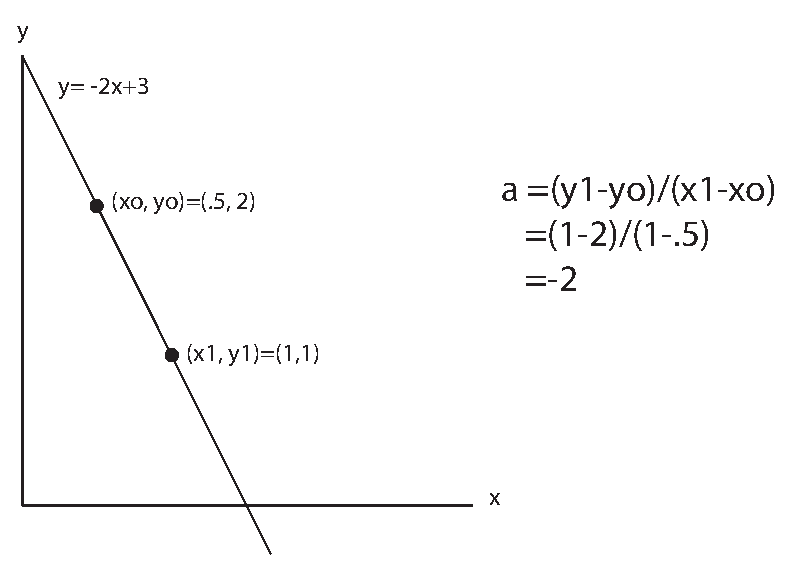
\includegraphics[scale = 0.4]{slope.eps}
\end{center}

\end{frame}



\begin{frame}
\frametitle{Slope of a Curve}
\begin{itemize}
\item Much of the time our functions are not straight lines.  In these cases, we add the notion of limits to our definition.
\item  Consider the slope at the point P.
\end{itemize}
\begin{center}
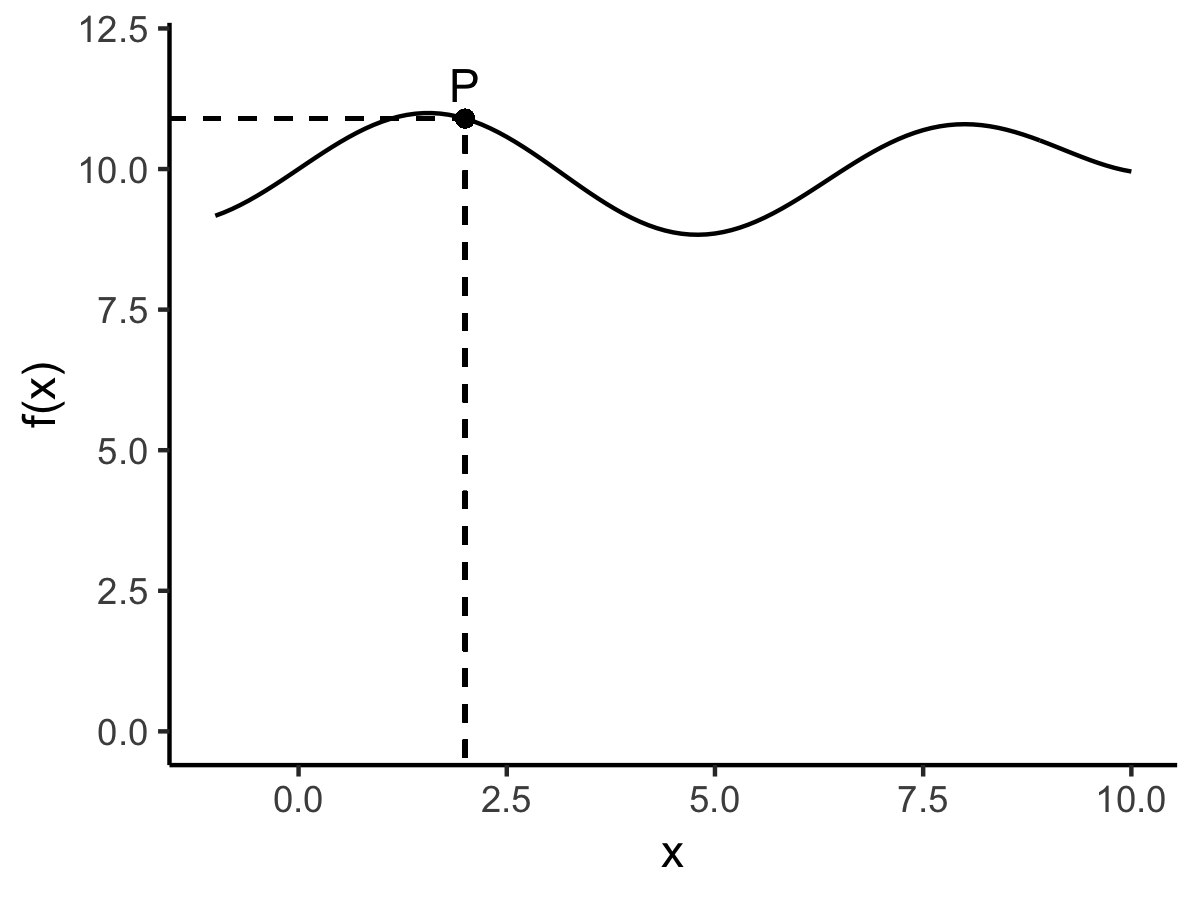
\includegraphics[width=3 in]{pointP.png}
\end{center}

\end{frame}

\begin{frame}
\frametitle{Slope of a Curve}
\begin{itemize}
\item Much of the time our functions are not straight lines.  In these cases, we add the notion of limits to our definition.
\item Consider the slope at the point P.
\end{itemize}
\begin{center}
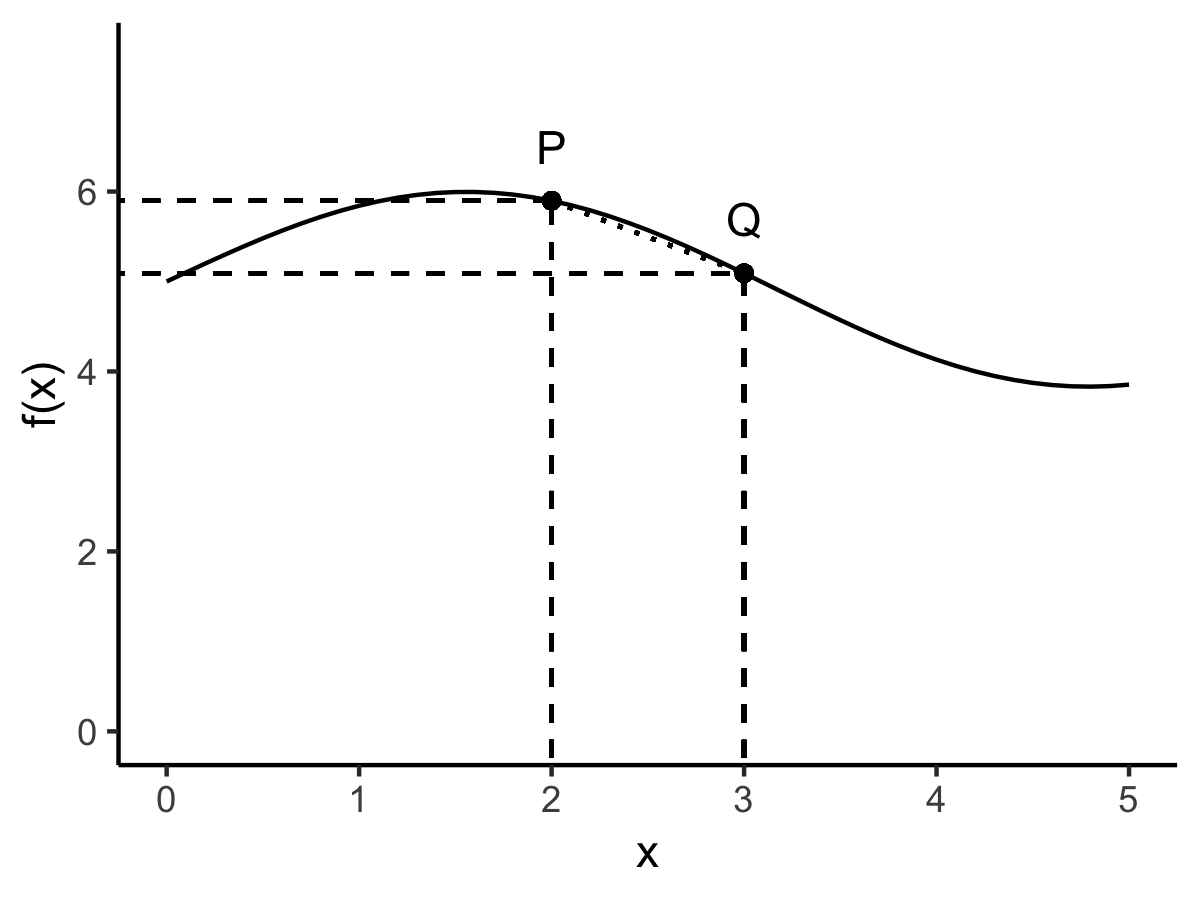
\includegraphics[width=3 in]{pointPandQ.png}
\end{center}

\end{frame}

\begin{frame}
\frametitle{Slope of a Curve}

The \textit{slope of the curve} $f(x)$ at point $P$ is the limit of the slope of the line between points $Q$ and $P$ as $Q\rightarrow P$ \pause

\begin{itemize}

\item Consider points $P=(x_0, f(x_0))$ and $Q=(x_1, f(x_1))$.\pause
\item Write $x_1=x_0+h$ so that we have $x_1\rightarrow x_0$ as $h\rightarrow 0$ \pause
\item[] $P=(x_0, f(x_0))$ and $Q=(x_0+h, f(x_0+h))$.\pause

\item[]
\end{itemize}
$$\frac{\text{rise}}{\text{run}}=\frac{y_{1} - y_{0}}{x_{1} - x_{0}} = \frac{f(x_{o} + h) - f(x_{0})}{x_{o} + h - x_{0}}=\frac{f(x_{o} + h) - f(x_{0})}{ h }$$ \pause

\ \\As $h \rightarrow 0$, $Q\rightarrow P$ and we have the \emph{derivative} of $f(x)$ at $x_{o}$.

\end{frame}



\begin{frame}
\frametitle{Derivative: Formal Definition}
Suppose $f:\mathbb{R} \rightarrow \mathbb{R}$. \pause \invisible<1>{Consider a measure rate of change at a point $x_{0}$ with a function $R(x)$, } \pause 
\begin{eqnarray}
\invisible<1-2>{R(x) & = & \frac{f(x) - f(x_{0}) }{ x- x_{0} } \nonumber } \pause 
\end{eqnarray}
\begin{itemize}
\invisible<1-3>{\item[-] $R(x)$ defines the rate of change. } \pause 
\invisible<1-4>{\item[-] A derivative will examine what happens with a small perturbation at $x_{0}$} 
\end{itemize}

\end{frame}



\begin{frame}
\frametitle{Derivative Definition}

\begin{defn}
Let $f:\mathbb{R} \rightarrow \mathbb{R}$.  If the limit
\begin{eqnarray}
\lim_{x\rightarrow x_{0}} R(x) & = & \frac{f(x) - f(x_{0}) }{x - x_{0}} \nonumber  \\
& = & f^{'}(x_{0}) \nonumber 
\end{eqnarray}
exists then we say that $f$ is \alert{differentiable} at $x_{0}$.\\  If $f^{'}(x_{0})$ exists for all $x \in \text{Domain}$, then we say that $f$ is differentiable. 
\end{defn}

\end{frame}



\begin{frame}
\frametitle{Derivative Examples}

\begin{itemize}
\item[-] Suppose $f(x) = x^2$ and consider $x_{0} = 1$.  Then, \pause 
\begin{eqnarray}
\lim_{x\rightarrow 1}R(x) & = & \lim_{x\rightarrow 1} \frac{x^2 - 1^2}{x - 1} \nonumber \pause \\
& = & \lim_{x\rightarrow 1} \frac{(x- 1)(x + 1) }{ x- 1} \nonumber \pause  \\
& = &  \lim_{x\rightarrow 1} x + 1 \nonumber \pause \\
& = & 2 \nonumber \pause 
\end{eqnarray}
\end{itemize}

\ \\The figure looks like:

\end{frame}



\begin{frame}
\frametitle{Derivative Examples}

\begin{figure}[!ht]
\centering
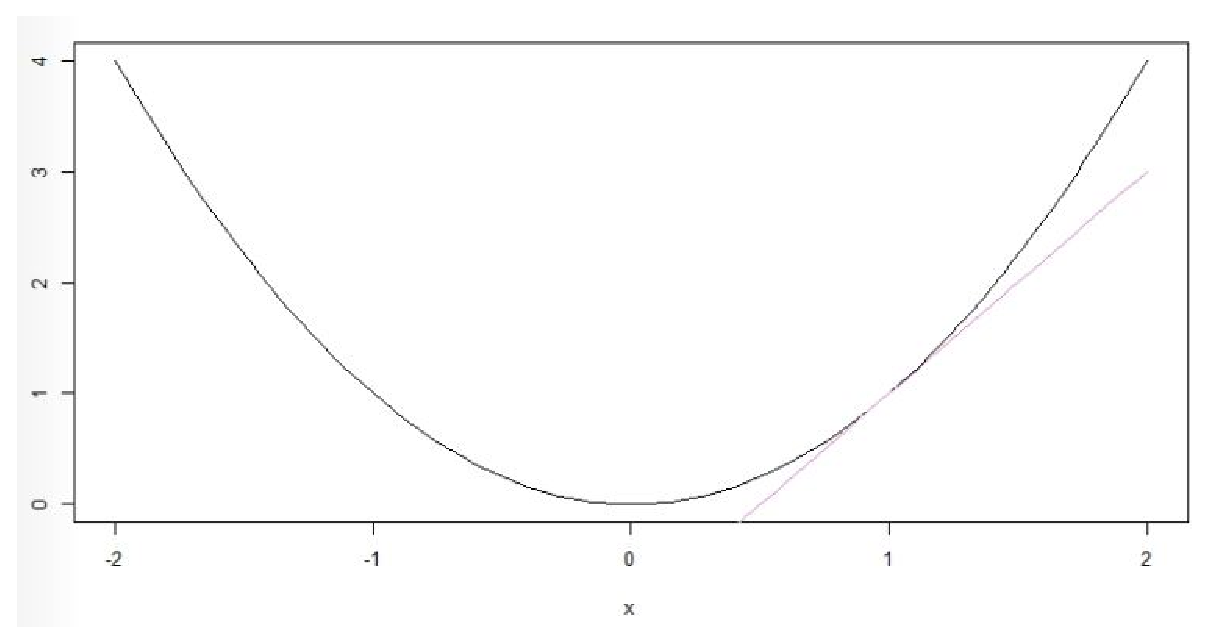
\includegraphics[scale = 0.5]{plsc43401_lec3_pic1}
\end{figure}

\end{frame}



\begin{frame}
\frametitle{Derivative Existence}

\begin{itemize}
\item[-] Not all functions have a derivative. \pause 
\item Suppose $f(x) = |x|$ and consider $x_{0} = 0$.  Then, \pause 
\begin{eqnarray}
\lim_{x\rightarrow 0} R(x) & = & \lim_{x\rightarrow 0} \frac{ |x| } {x} \nonumber  \pause 
\end{eqnarray}
$\lim_{x \rightarrow 0^{-}} R(x) = -1$ \pause , but $\lim_{x \rightarrow 0^{+}} R(x) = 1$. \pause
\ \\Given this, we say, $|x|$ not differentiable at $0$.



\end{itemize}

\end{frame}



\begin{frame}
\frametitle{Graph of $|x|$}

\begin{figure}[!ht]
\centering
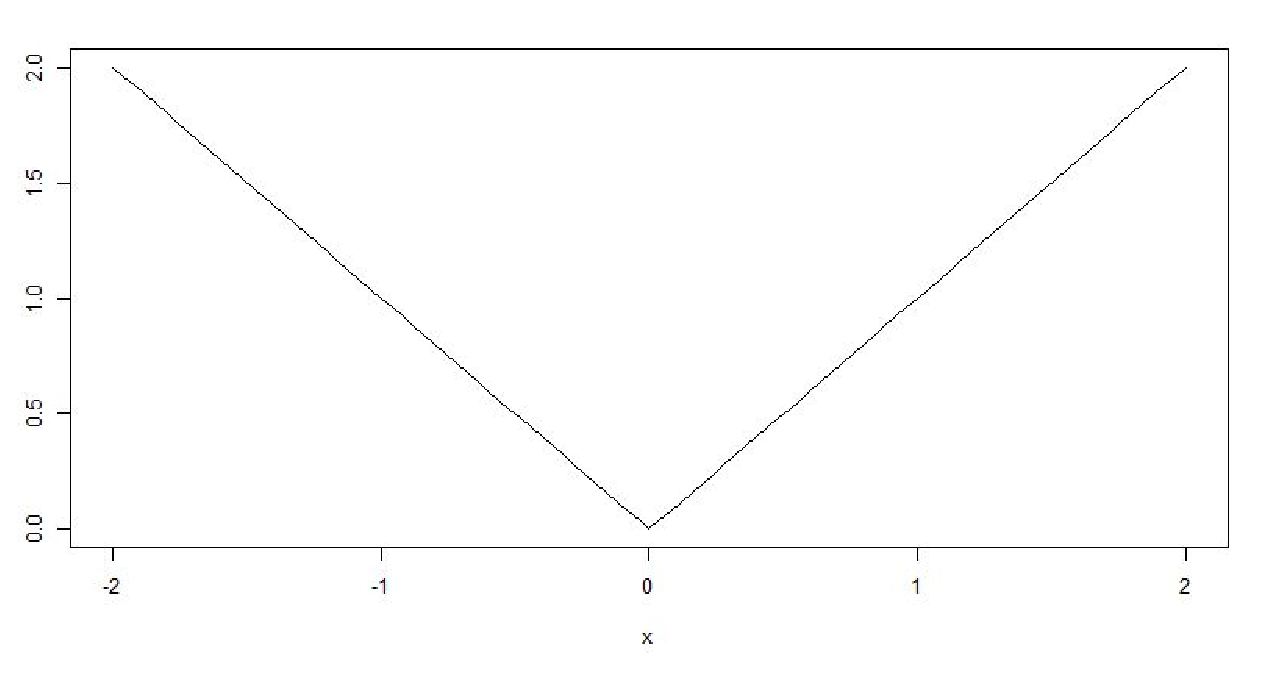
\includegraphics[scale = 0.5]{plsc43401_lec3_pic2}
\end{figure}

\end{frame}


\begin{frame}

\begin{itemize}
\item \textcolor{mygray}{Derivative}
\item \textcolor{myblack}{Derivative and Continuity}
\item \textcolor{mygray}{Derivative Rules}
\item \textcolor{mygray}{Mean Value Theorem}
\item \textcolor{mygray}{Second Derivatives}
\end{itemize}

\end{frame}



\begin{frame}
\frametitle{Derivative and Continuity}

$|x|$ is continuous but not differentiable. If a function is differentiable, then it is continuous.\pause

\begin{thm} Let $f:\mathbb{R} \rightarrow \mathbb{R}$ be differentiable at $x_{0}$.  Then $f$ is continuous at $x_{0}$.
\end{thm}
\pause
Our proof strategy: 
\begin{itemize}
\item We need $\lim_{x\rightarrow x_{0}} f(x) = f(x_{0})$ (recall last lecture).
\item Use direct proof: Start with f(x) that is differentiable.
\item Manipulate till we get the formula for the rate of change $R(x) =\frac{ f(x) - f(x_{0})}{(x- x_{0})}$. 
\item Take the limit, use limit properties, get $f(x_{0}).$
\end{itemize}
 \end{frame}



\begin{frame}
\frametitle{Proof of Derivative and Continuity}
\begin{proof}
Consider some differentiable $f(x)$: \pause 
\begin{eqnarray}
f(x) & =& f(x) -f(x_{0} )+f(x_{0}) \nonumber  \pause  \\
f(x) & = & \frac{ f(x) - f(x_{0})}{(x- x_{0})} (x - x_{0} ) + f(x_{0} )\nonumber  \pause  \\
& = & R(x) (x - x_{0} ) + f(x_{0} ) \nonumber \pause 
	\end{eqnarray}
Remember: if $f(x)$ is continuous at $x_{0}$ then, $\lim_{x\rightarrow x_{0}} f(x) = f(x_{0})$.  \pause 
\begin{eqnarray}
\lim_{x\rightarrow x_{0}} f(x) & = & \lim_{x\rightarrow x_{0} } [R(x) (x - x_{0} ) + f(x_{0}) ] \nonumber \\ \pause 
& = & \left(\lim_{x\rightarrow x_{0} } R(x) \right)\left(\lim_{x\rightarrow x_{0}} (x - x_{0}) \right)  + \lim_{x\rightarrow x_{0}} f(x_{0} ) \nonumber \\ \pause 
& = & f^{'}(x_{0} ) 0 + f(x_{0})  \nonumber \\\pause
& = &f(x_{0} ) \nonumber
	\end{eqnarray}

\end{proof}

\end{frame}



\begin{frame}

\begin{itemize}
\item \textcolor{mygray}{Derivative}
\item \textcolor{mygray}{Derivative and Continuity}
\item \textcolor{myblack}{Derivative Rules}
\item \textcolor{mygray}{Mean Value Theorem}
\item \textcolor{mygray}{Second Derivatives}
\end{itemize}

\end{frame}


\begin{frame}
\frametitle{Useful Derivative Rules}

Suppose $a$ is some constant, $f(x)$ and $g(x)$ are functions \pause 
\begin{eqnarray}
f(x) = x & ; & f^{'}(x) = 1 \nonumber \\ \pause 
f(x) = a x^{k} & ; & f^{'}(x) = (a) (k) x ^{k-1} \nonumber \\ \pause 
f(x) = e^{x } & ; & f^{'} (x) = e^{x} \nonumber \\ \pause 
f(x) = \sin(x) & ; & f^{'} (x) = \cos (x) \nonumber \\ \pause 
f(x) = \cos(x) & ; & f^{'} (x) = - \sin(x) \nonumber \\ \pause 
f(x) = log(x) & ; & f^{'} (x) = \frac{1}{x} \nonumber 
\end{eqnarray}

\end{frame}

\begin{frame}
\frametitle{Proof the $exp(x)\equiv e^x$ is its own derivative}

Recall $e^x=\sum_{n=0}^{\infty} \frac{x^n}{n!}$

\begin{eqnarray}
exp'(x) &=& \lim_{h\rightarrow 0} \frac{exp(x+h)-exp(x)}{h} \nonumber\\\pause
&=& \lim_{h\rightarrow 0} \frac{exp(x)exp(h)-exp(x)}{h}\nonumber\\\pause
&=& exp(x)\lim_{h\rightarrow 0} \frac{exp(h)-1}{h}\nonumber
\end{eqnarray}
\pause

\end{frame}

\begin{frame}
\frametitle{Proof the $exp(x)\equiv e^x$ is its own derivative (cont.)}


\begin{eqnarray}
\frac{exp(h)-1}{h}&=&\frac{\sum_{n=0}^{\infty} \frac{h^n}{n!}-1}{h}\nonumber\\\pause
&=&\frac{[\frac{h^0}{0!}+\frac{h^1}{1!}+\frac{h^2}{2!}...]-1}{h}\nonumber\\\pause
&=&\frac{[\frac{1}{1}+\frac{h^1}{1}+\frac{h^2}{2}...]-1}{h}\nonumber\\\pause
&=&\frac{[h+\frac{h^2}{2}...]}{h}\nonumber\\\pause
&=&1+\frac{h}{2}+\frac{h^2}{3}...\nonumber
\end{eqnarray}


\end{frame}

\begin{frame}
\frametitle{Proof the $exp(x)\equiv e^x$ is its own derivative (finish)}



\begin{eqnarray}
exp'(x) &=& \lim_{h\rightarrow 0} \frac{exp(x+h)-exp(x)}{h} \nonumber\\
&=& exp(x)\lim_{h\rightarrow 0} \frac{exp(h)-1}{h}\nonumber\\
&=& exp(x)\lim_{h\rightarrow 0}[1+\frac{h}{2}+\frac{h^2}{3}...]\nonumber\\\pause
&=& exp(x)*1\nonumber\\ \pause
exp'(x)&=& exp(x)\quad \qed\nonumber
\end{eqnarray}

\end{frame}


\begin{frame}
\frametitle{Derivative in Political Economy}

\begin{itemize}
\item The policy space is $\mathbb{R}$ \pause
\item A person (voter?)  has an ``ideal point" $p\in \mathbb{R}$ \pause
\item Person prefers policies that are closer to his/her ideal point: receives utility  from policy $x$ 
\end{itemize}
$$u(x)=-(x-p)^2$$
$$u^\prime(x)=2p-2x$$

\end{frame}


\begin{frame}
\frametitle{Algebra of Derivatives}

\begin{thm} Suppose $f:\mathbb{R} \rightarrow \mathbb{R}$ and $g:\mathbb{R} \rightarrow \mathbb{R}$ and both are differentiable at $x_{0} \in \mathbb{R}$.  Then, \pause 
\begin{itemize}
\item[i)] $h(x) = f(x) + g(x)$ is differentiable at $x_{0}$ and \pause 
\begin{eqnarray}
h^{'} (x_{0}) & = & f^{'}(x_{0}) + g^{'} (x_{0}) \nonumber \pause 
\end{eqnarray}
\item[ii)] $h(x) = f(x) g(x) $ is differentiable at $x_{0}$ and \pause 
\begin{eqnarray}
h^{'}(x_{0}) & = & f^{'}(x_{0}) g(x_{0}) + g^{'}(x_{0}) f(x_{0}) \nonumber  \pause 
\end{eqnarray}
\item[iii)] $h(x)  = \frac{f(x) }{g(x) }$ with $g(x) \neq 0$ then, \pause 
\begin{eqnarray}
h^{'}(x_{0}) & = &  \frac{f^{'}(x_{0}) g(x_{0}) - g^{'}(x_{0}) f(x_{0})} {g(x_{0})^2} \nonumber
\end{eqnarray}
\end{itemize}
\end{thm}

\end{frame}










\begin{frame}
\frametitle{Algebra of Derivatives: Examples}

\begin{itemize}
\item[1)] $f(x)= x^3 + 5 x^2  + 4 x$ \pause
\begin{eqnarray}
f'(x) & = & 3 x^2 + 5 * 2x + 4 \nonumber \pause \\
      & = & 3 x^2 + 10x + 4 \nonumber \pause
\end{eqnarray}
     
\end{itemize}

\begin{itemize}
\item[2)] $f(x) = sin(x) x^3$ \pause
\begin{eqnarray}
f'(x) & = & cos(X)  x^3 + sin(x)  3 x^2 \nonumber \pause \\
& = & cos(X)  x^3 + 3 sin(x)  x^2 \nonumber \pause
\end{eqnarray}
\end{itemize}

\begin{itemize}
\item[3)] $f(x) = \frac{e^{x} }{x^3}$ \pause
\begin{eqnarray}
f'(x) & = & \frac{e^{x}  x^{3} - e^{x}  3 x^{2} }{x^6} \nonumber \pause \\
& = & \frac{e^{x}  x^{3} - 3 e^{x} x^{2} }{x^6} \nonumber
\end{eqnarray}

\end{itemize}

\end{frame}



\begin{frame}
\frametitle{Chain Rule} 
Common to have functions in functions
\begin{eqnarray}
f(x) & = & \frac{e^{ - \frac{(x - \mu)^2}{2 \sigma^2}}}{\sqrt{2 \pi }  } \nonumber \\
		& = & \frac{f (g(x)) } {\sqrt{2 \pi}} \nonumber 
\end{eqnarray}

\ \\where $f(x) = e ^{- g(x)}$, $g(x) = \frac{(x - \mu)^2}{2 \sigma^2}$ \pause

To deal with this, we use the \alert{chain rule} \pause

\begin{thm} 
Suppose $g: \mathbb{R} \rightarrow \mathbb{R}$ and $f: \mathbb{R} \rightarrow \mathbb{R}$. Suppose both $f(x)$ and $g(x)$ are differentiable at $x_{0}$.  Define $h(x) = g(f(x))$.  Then, 
\begin{eqnarray}
h^{'}(x_{0}) & = & g^{'}(f(x_{0}))f^{'}(x_{0}) \nonumber 
\end{eqnarray}
\end{thm}

\end{frame}


\begin{frame}
\frametitle{Examples of Chain Rule}
\begin{itemize}
\item[-] $h(x) = e^{2x}$.  $g(x) = e^{x}$.  $f(x) = 2x$.  \pause So $h(x) = g(f(x)) = g(2x) = e^{2x}$.  Taking derivatives, we have \pause
\begin{eqnarray}
h^{'}(x) & = & g^{'}(f(x))f^{'}(x) = e^{2x}2 \nonumber 
\end{eqnarray} \pause
\item[-] $h(x) = \log(\cos(x) )$.  $g(x) = log(x)$.  $f(x) = \cos(x)$. \pause\\
 $h(x) = g(f(x)) = g( \cos(x)) = log(\cos(x))$  \pause
\begin{eqnarray}
h^{'}(x) & = & g^{'}(f(x))f^{'}(x) = \frac{-1}{\cos(x)} \sin(x) = -\tan (x) \nonumber 
\end{eqnarray}
\end{itemize}

\end{frame}

\begin{frame}
\frametitle{Derivative of a fraction}

\begin{itemize}
\item We can use the chain rule to show that the product rule and the quotient rule are the same:
\begin{eqnarray}
\frac{f(x) }{g(x) }& = &f(x) (g(x))^{-1} \nonumber \pause\\
 \frac{d f(x) (g(x))^{-1}}{dx}& = & f^{'}(x) (g(x))^{-1} +\frac{d(g(x))^{-1}}{dx} f(x)\nonumber  \pause\\
& = & f^{'}(x) (g(x))^{-1} +(-1)g(x)^{-2}g'(x) f(x) \nonumber  \pause\\
    & = & \frac{f^{'}(x)}{ g(x)} - \frac{g'(x) f(x)}{g(x)^{2}} \nonumber  \pause\\
        & = & \frac{f^{'}(x)g(x)-g'(x) f(x)}{g(x)^{2}} \nonumber 
  \end{eqnarray}
 \end{itemize}

\end{frame}



\begin{frame}

\begin{itemize}
\item \textcolor{mygray}{Derivative}
\item \textcolor{mygray}{Derivative Rules}
\item \textcolor{myblack}{Mean Value Theorem}
\item \textcolor{mygray}{Second Derivatives}
\end{itemize}

\end{frame}



\begin{frame}
\frametitle{Relative Maxima, Minima and Derivatives}

\begin{figure}[!ht]
\centering
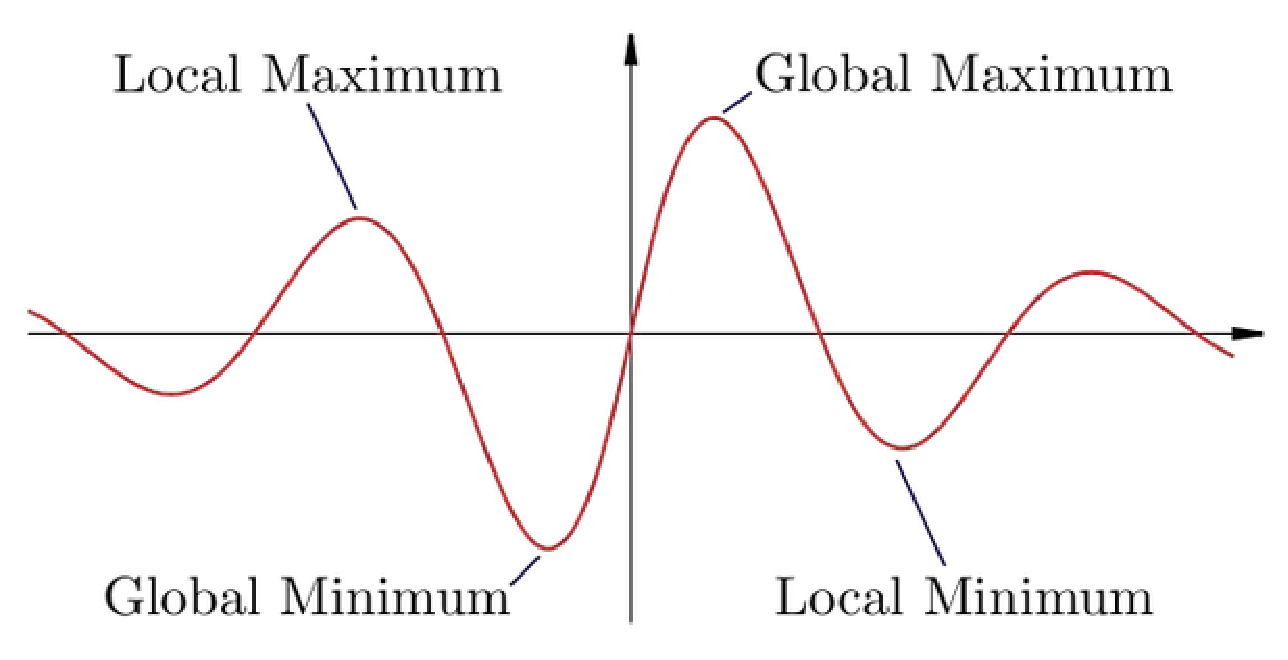
\includegraphics[scale = 0.36]{plsc43401_lec3_pic3}
\end{figure}
\begin{itemize}
\item We use derivatives to find the maxima and minima.\pause
\item We need maxima (or minima) for statistical inference (what is \textbf{most} likely), \pause modeling choices (what is \textbf{most preferred}), \pause and for modeling systems (what is \textbf{stable}).\pause
\item The connection between maxima and derivatives is shown with the Mean Value Theorem (MVT).
\item To get there we prove a special case of MVT called ``Rolle's Theorem.''
\end{itemize}
\end{frame}



\begin{frame}
\frametitle{Aside: Naming Conventions of Theorems}

\begin{itemize}
\item Stigler's Law of Eponomy.\pause
\item[-] ``No scientific discovery is named for the person who discovered it.''
\item Rolle's Theorem was proved by Cauchy (1823), but first stated by a 12th century Indian mathematician Bhaskara II
\end{itemize}
\end{frame}


\begin{frame}
\frametitle{Derivatives and local maxima/minima}

\begin{thm} Rolle's Theorem Suppose $f:[a,b] \rightarrow \mathbb{R}$ and $f$ is continuous on $[a,b]$ and differentiable on $(a,b)$.  Then if $f(a) = f(b) = 0$, there is $c \in (a, b)$ such that $f^{'}(c) = 0$.  \end{thm}\pause

\begin{itemize}
\item This claims that fixing two points at the same level, the function has to curve back at some point (it hits a max or min), where the tangent is flat.\pause
\item Proof intuition:\pause
\begin{itemize}
\item Consider a relative maximum $c$. \pause
\item Find the left-hand (approaching from below) and right-hand limits (approaching from the above).\pause
\item Show that the left hand limit can't be positive, and the right hand limit can't be negative.
\item Then all that is left is 0.
\end{itemize}
\end{itemize}
\end{frame}


\begin{frame}{Formal Proof of Rolle's Theorem}
Suppose $f:[a,b] \rightarrow \mathbb{R}$ and $f$ is continuous on $[a,b]$ and differentiable on $(a,b)$.  \pause
If $f(x)=0$ for all x, then $f'(x)=0$ and we are done.\\ \pause
If not, there is some c that is either a min or a max.\\
If it is a max, then $f(x)-f(c)\leq0$
By the definition of differentiability: \pause
\begin{eqnarray}
\lim_{x \rightarrow c^{-}} \frac{f(x) - f(c ) }{x - c } & = & f^{'}(c)\leq0 \nonumber \\\pause
\lim_{x \rightarrow c^{+}} \frac{f(x) - f(c) } {x - c }  &  =  & f^{'}(c)\geq0  \nonumber \pause
\end{eqnarray}

In order for these two limits to be equal, \\
$$\lim_{x \rightarrow c^{-}} \frac{f(x) - f(c) }{x -c}  = \lim_{x \rightarrow c^{+}} \frac{f(x) - f(c) } {x - c} $$
It must be that: $f^{'}(c) = 0$.  

\end{frame}



\begin{frame}
\frametitle{Mean Value Theorem} 

\begin{thm} If $f:[a,b] \rightarrow \mathbb{R}$ is continuous on $[a,b]$ and differentiable on $(a,b)$, then there is a $c \in (a,b)$ such that 

\begin{eqnarray}
f^{'}(c) & = & \frac{f(b) - f(a) } { b - a} \nonumber 
\end{eqnarray}
\end{thm}\pause

\begin{itemize}
\item That is, if there is a line connecting two points of a function, the slope will be equal to the derivative somewhere between the two points.
\item The proof strategy is to set up for an application of Rolle's theorem.
\end{itemize}
\end{frame}




\begin{frame}
\frametitle{Proof of Mean Value Theorem} 
Consider $f(x)$ as your differentiable function.  Construct a new function:

$$g(x)=f(x)-\frac{(f(b)-f(a))}{b-a}(x-a)$$\pause
$$\text{Note that: }g(a)=f(a)$$\pause 
\begin{eqnarray}
g(b)&=&f(b)-\frac{(f(b)-f(a))(b-a)}{b-a} \nonumber \\ \pause
&=&f(a)\nonumber\pause 
\end{eqnarray}
So g(x) is like f(x), in that if you evaluate it at $a$ we get $f(a)$, but if you evaluate it at $b$ you still get $f(a)$.  This means it starts and ends and the same place, so it must turn around.
\end{frame}


\begin{frame}
\frametitle{Intuition for Proof Strategy} 

$$g(x)=f(x)-\frac{(f(b)-f(a))}{b-a}(x-a)$$\pause
For instance:

\begin{figure}[!ht]
\centering
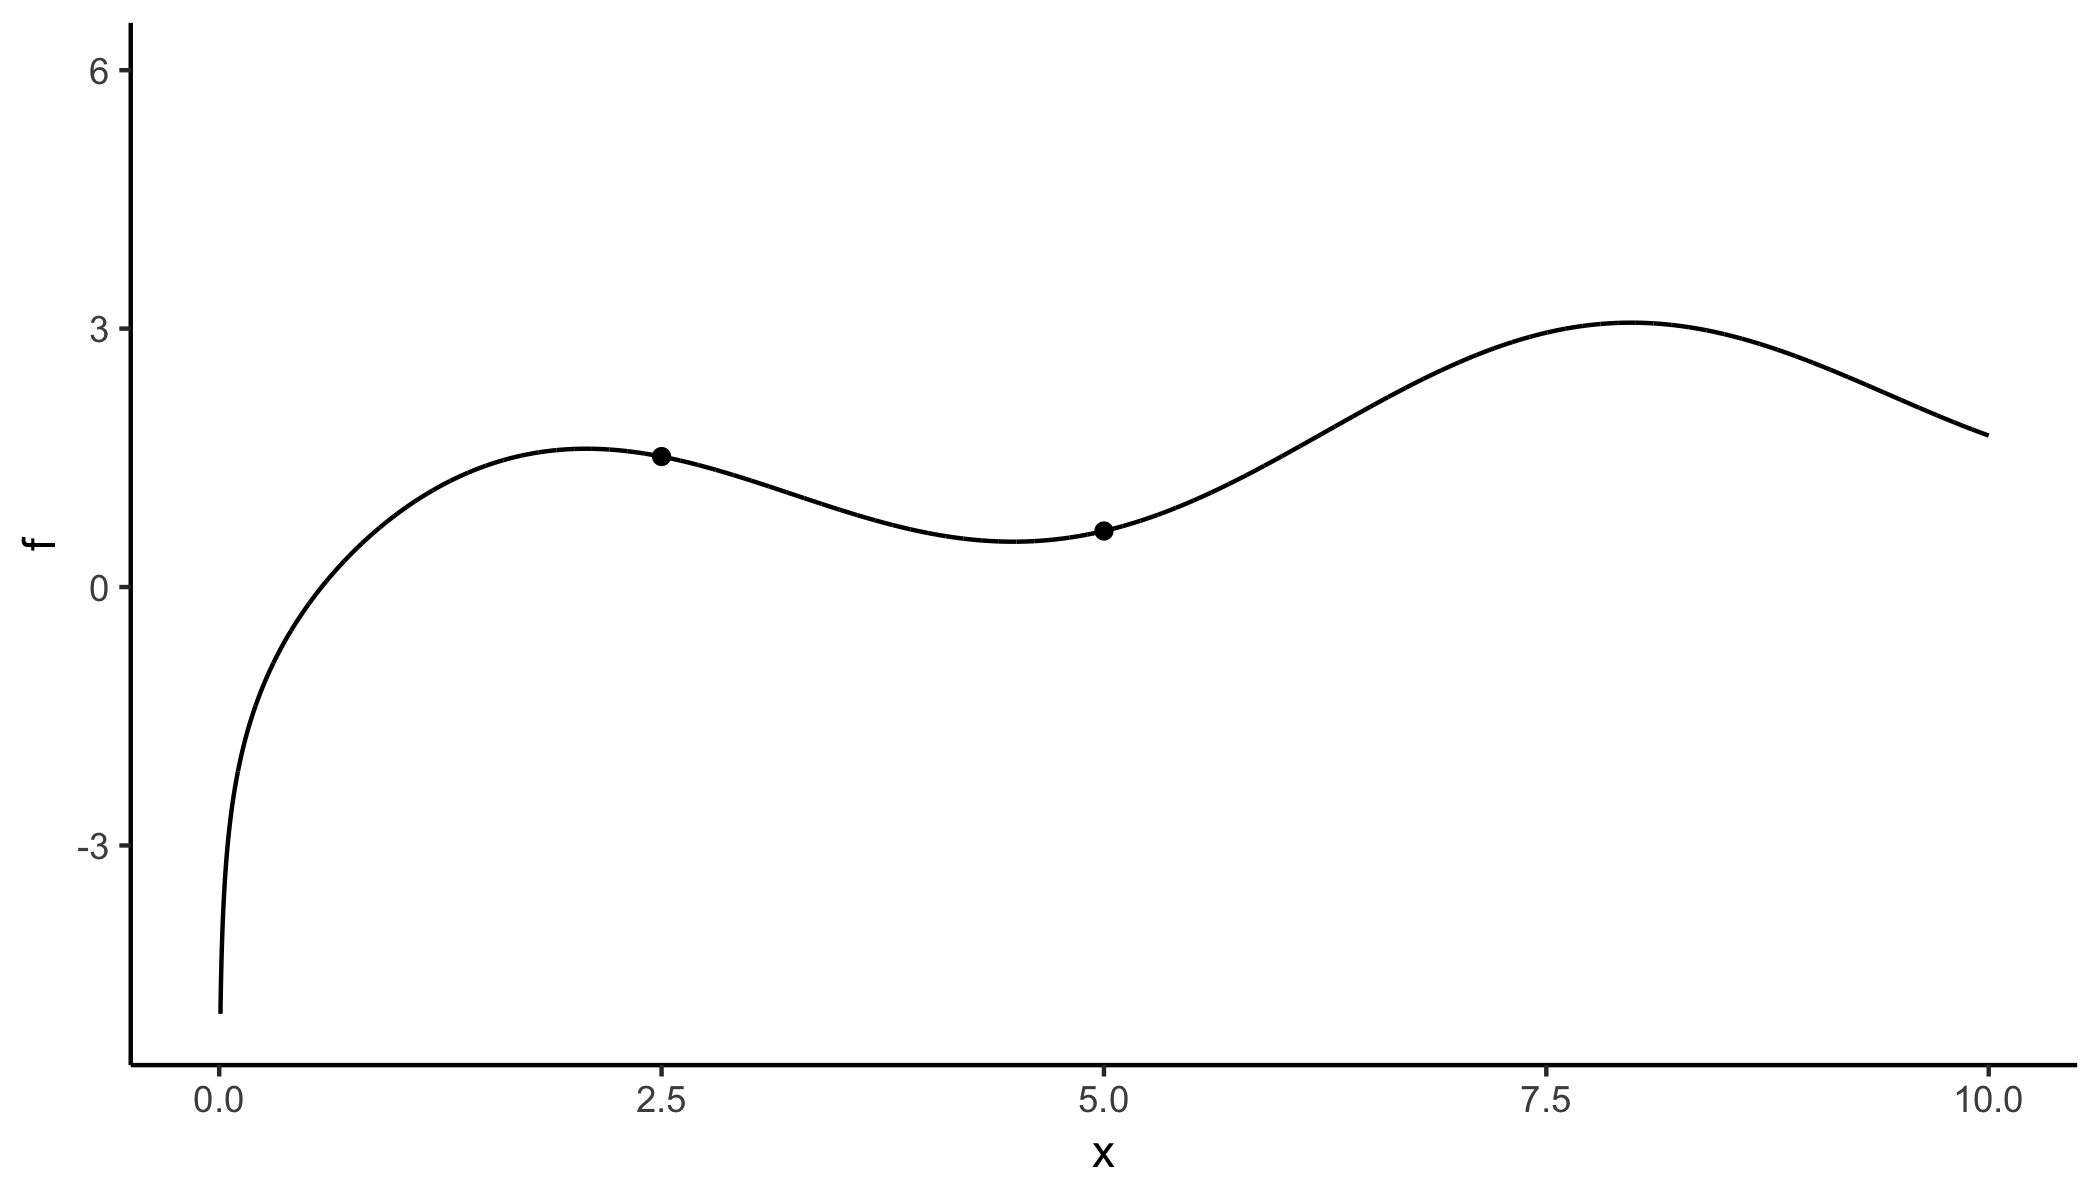
\includegraphics[width=3 in]{fig1.png}
\end{figure}
\end{frame}




\begin{frame}
\frametitle{Intuition for Proof Strategy} 

$$g(x)=f(x)-\frac{(f(b)-f(a))}{b-a}(x-a)$$
For instance:

\begin{figure}[!ht]
\centering
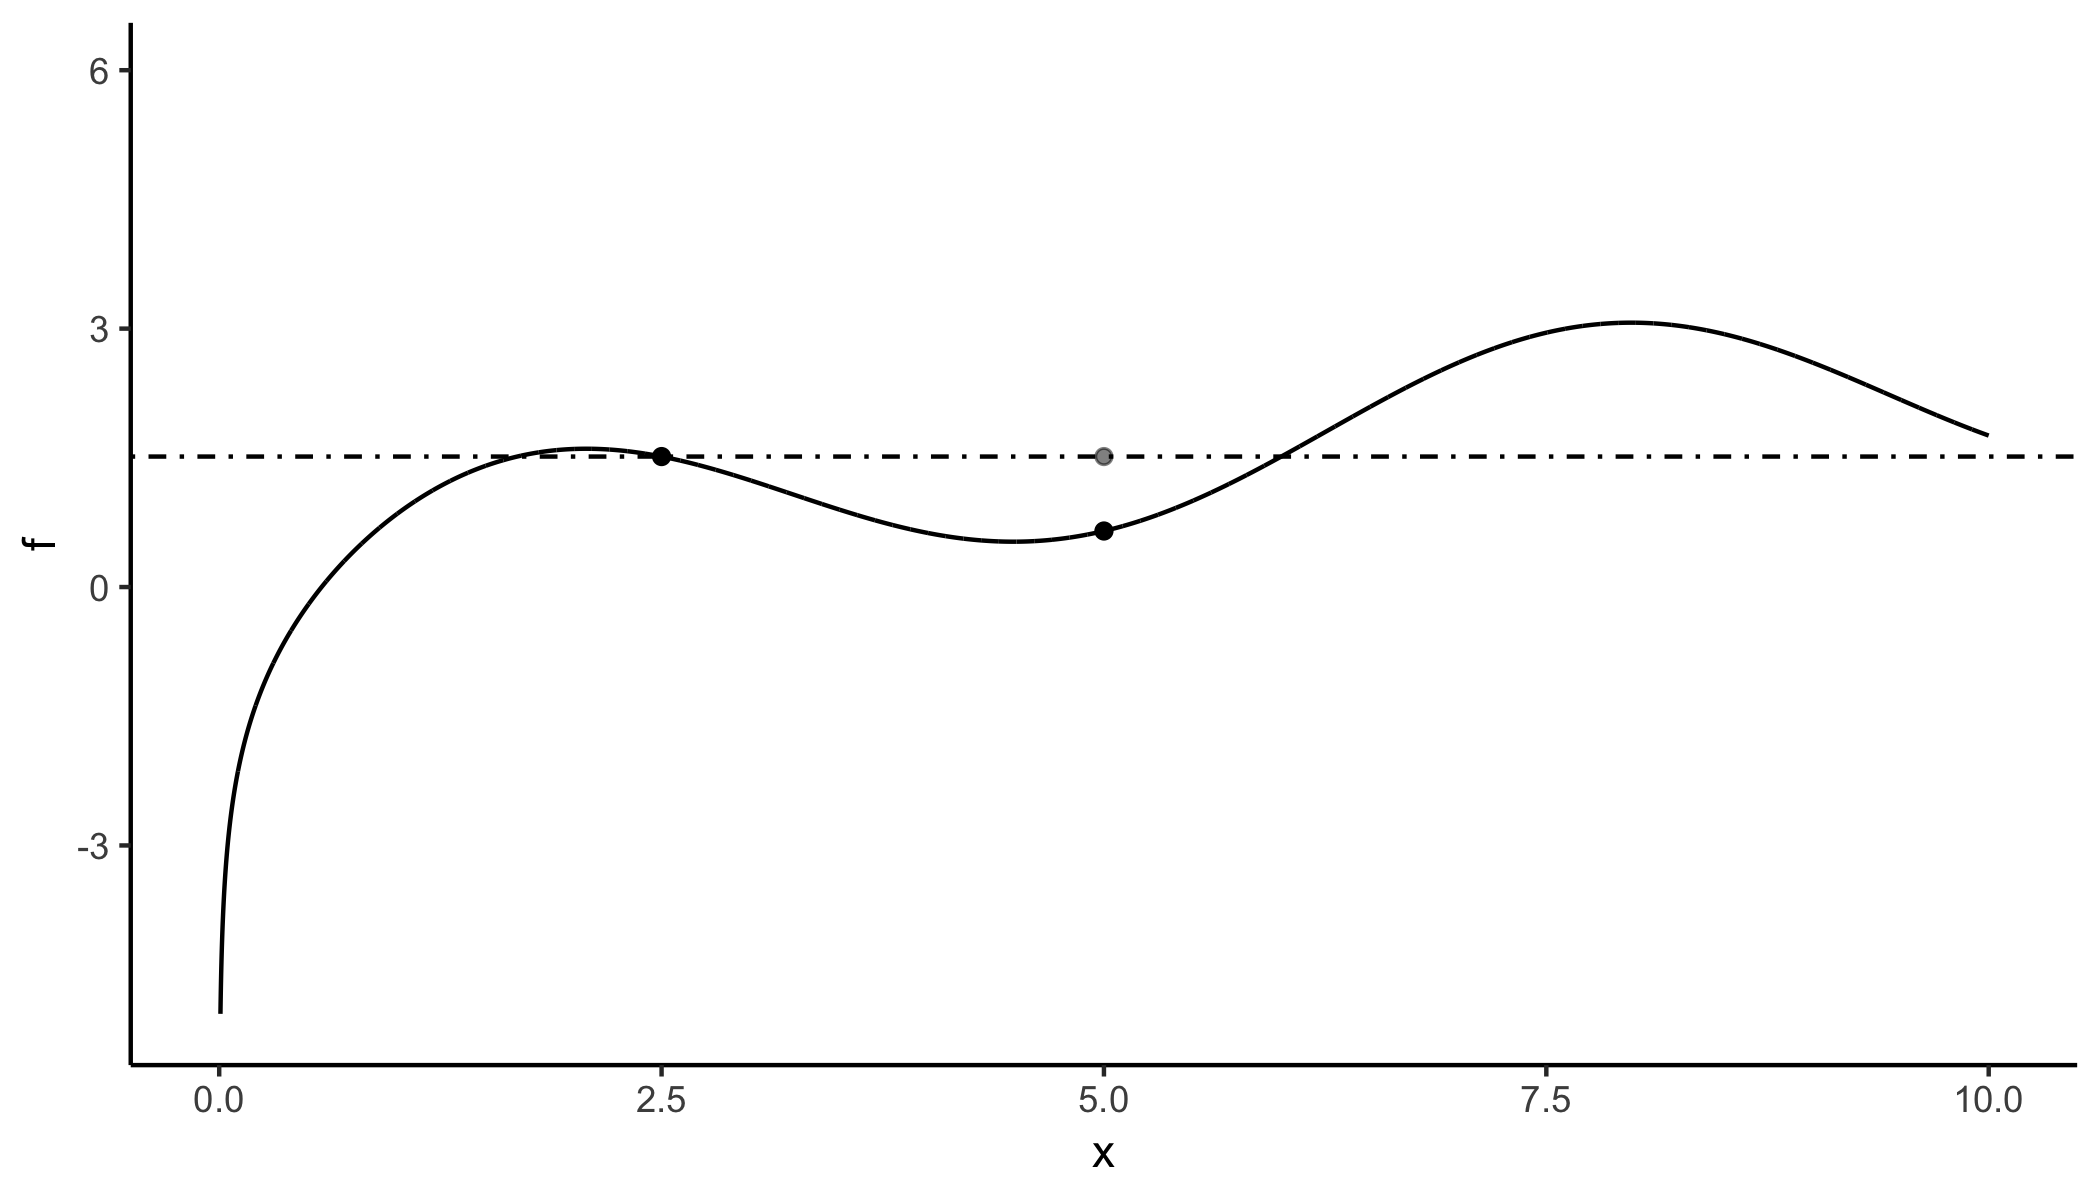
\includegraphics[width=3 in]{fig2.png}
\end{figure}
\end{frame}


\begin{frame}
\frametitle{Intuition for Proof Strategy} 

$$g(x)=f(x)-\frac{(f(b)-f(a))}{b-a}(x-a)$$
For instance:

\begin{figure}[!ht]
\centering
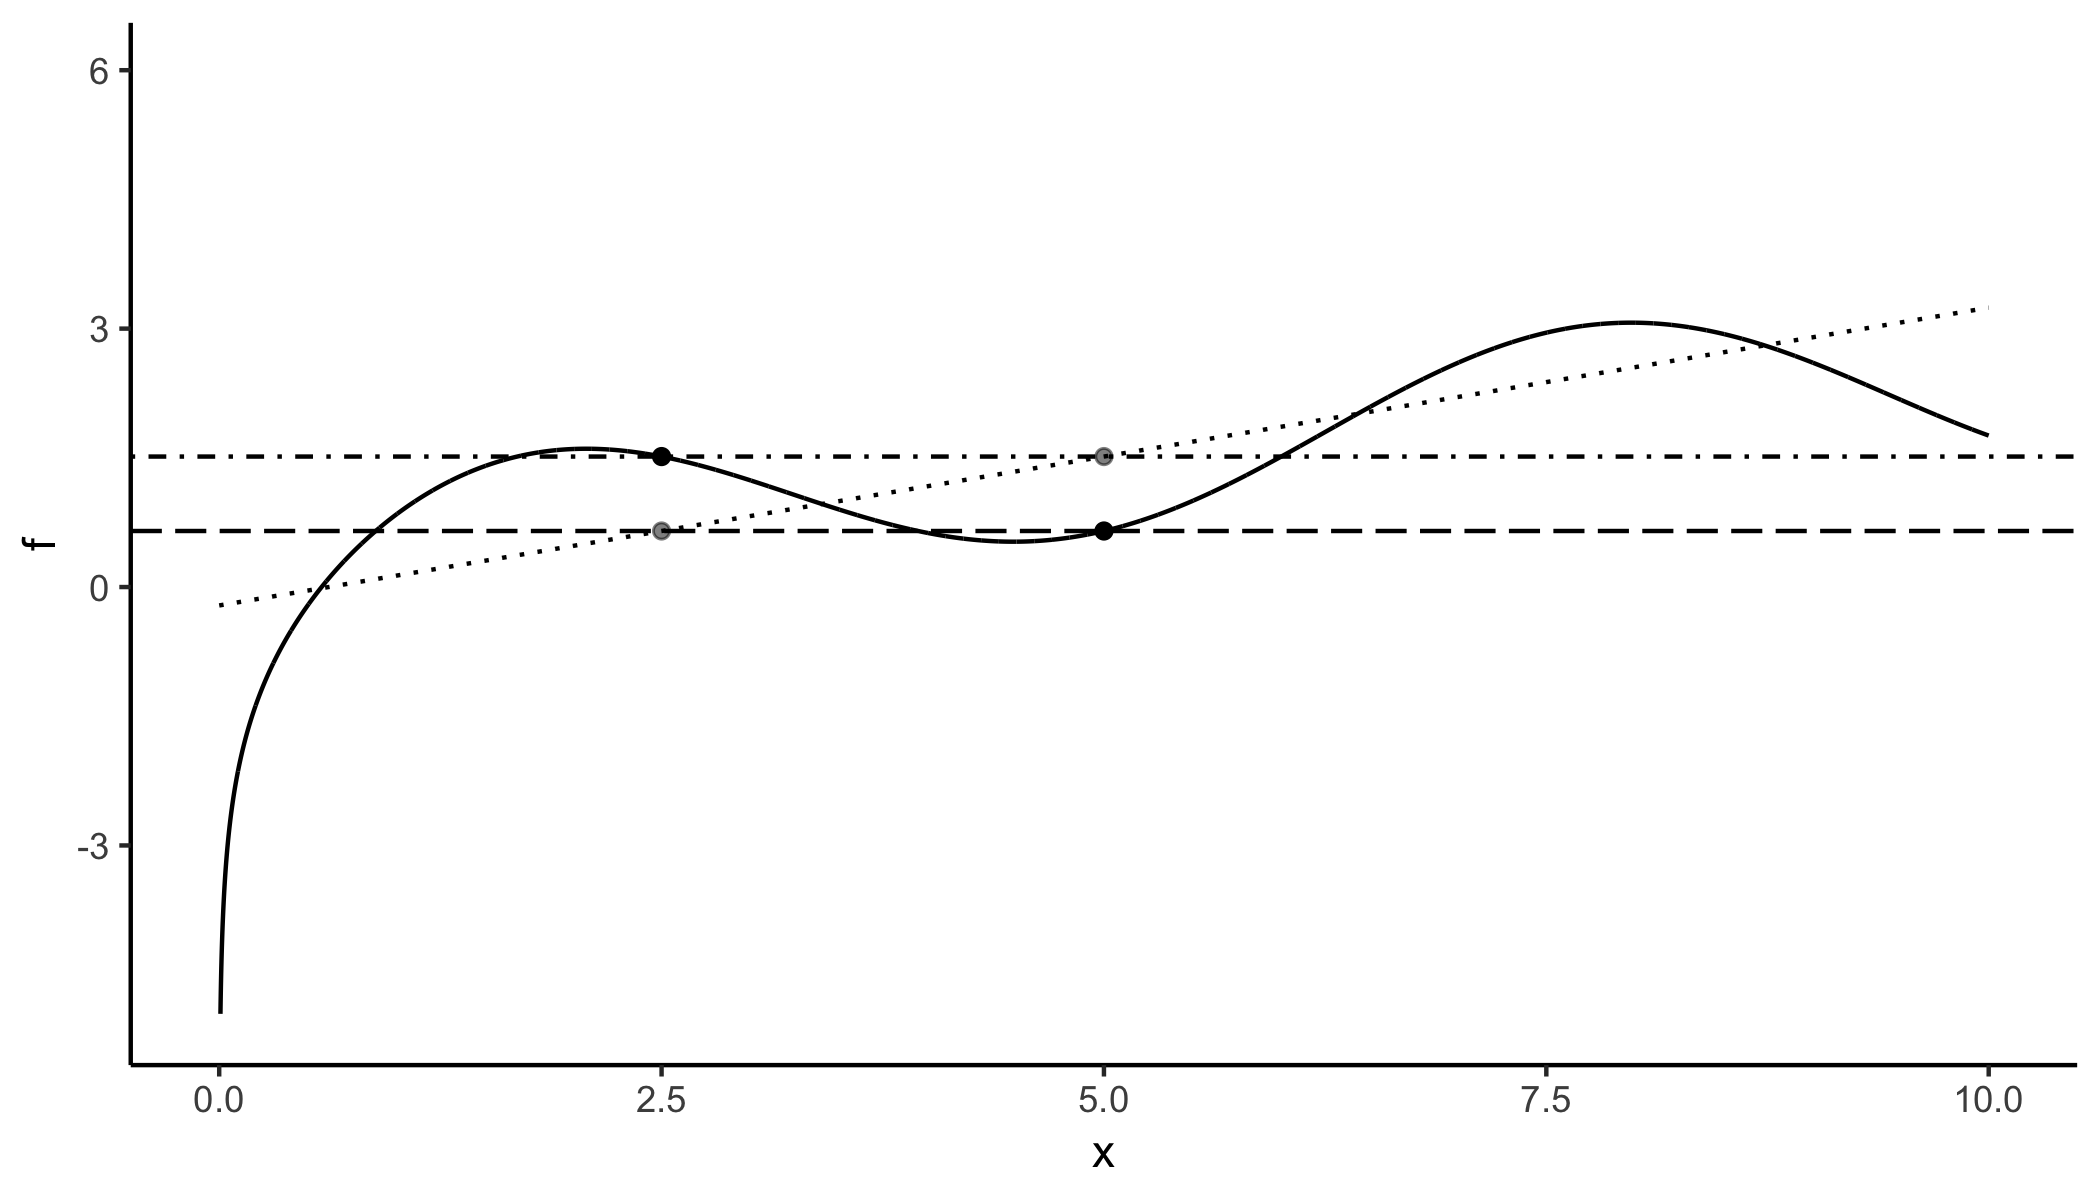
\includegraphics[width=3 in]{fig3.png}
\end{figure}
\end{frame}


\begin{frame}
\frametitle{Intuition for Proof Strategy} 

$$g(x)=f(x)-\frac{(f(b)-f(a))}{b-a}(x-a)$$
For instance:

\begin{figure}[!ht]
\centering
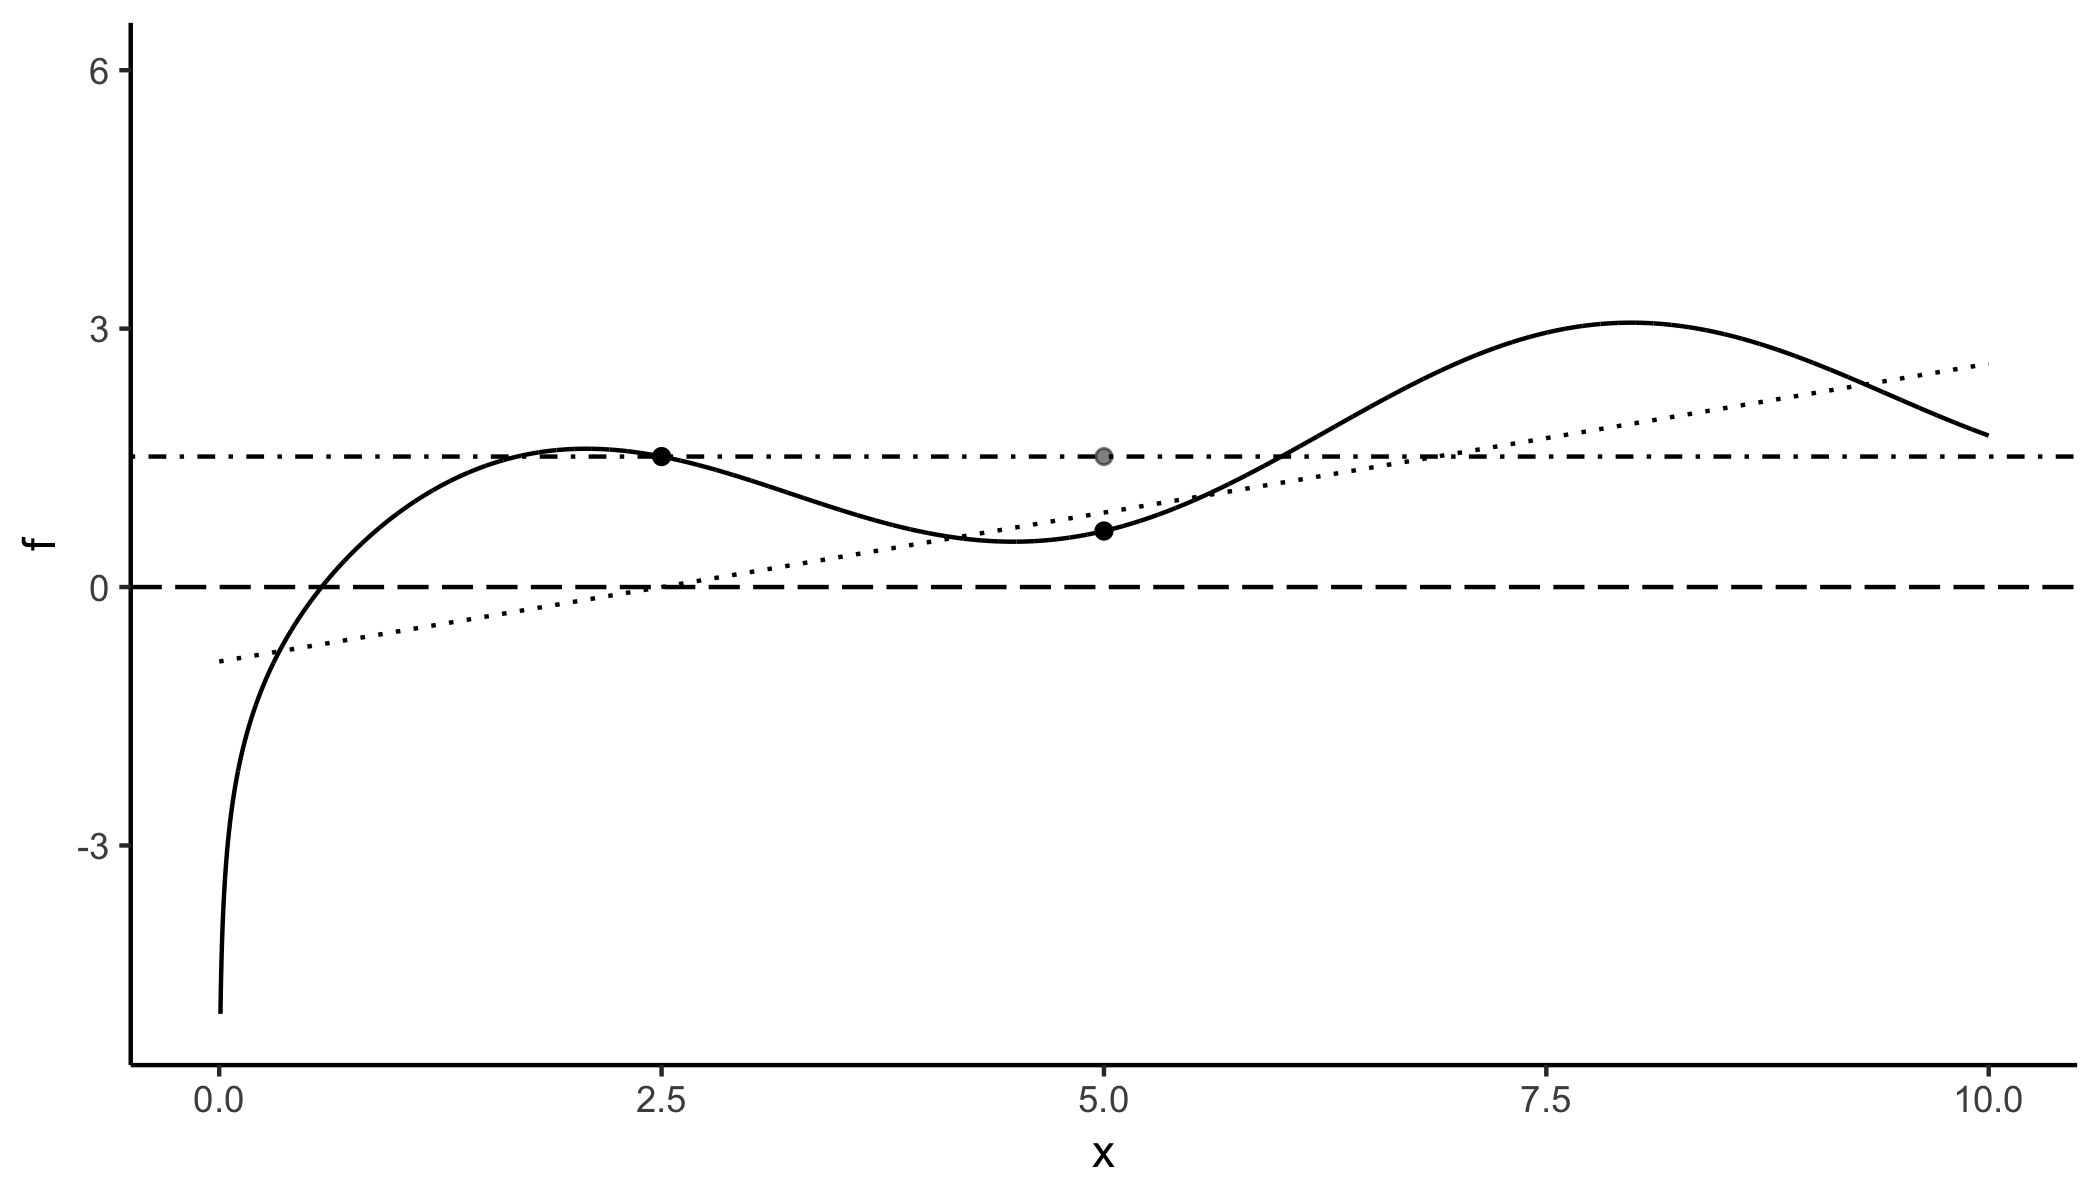
\includegraphics[width=3 in]{fig4.png}
\end{figure}
\end{frame}



\begin{frame}
\frametitle{Intuition for Proof Strategy} 

$$g(x)=f(x)-\frac{(f(b)-f(a))}{b-a}(x-a)$$
For instance:

\begin{figure}[!ht]
\centering
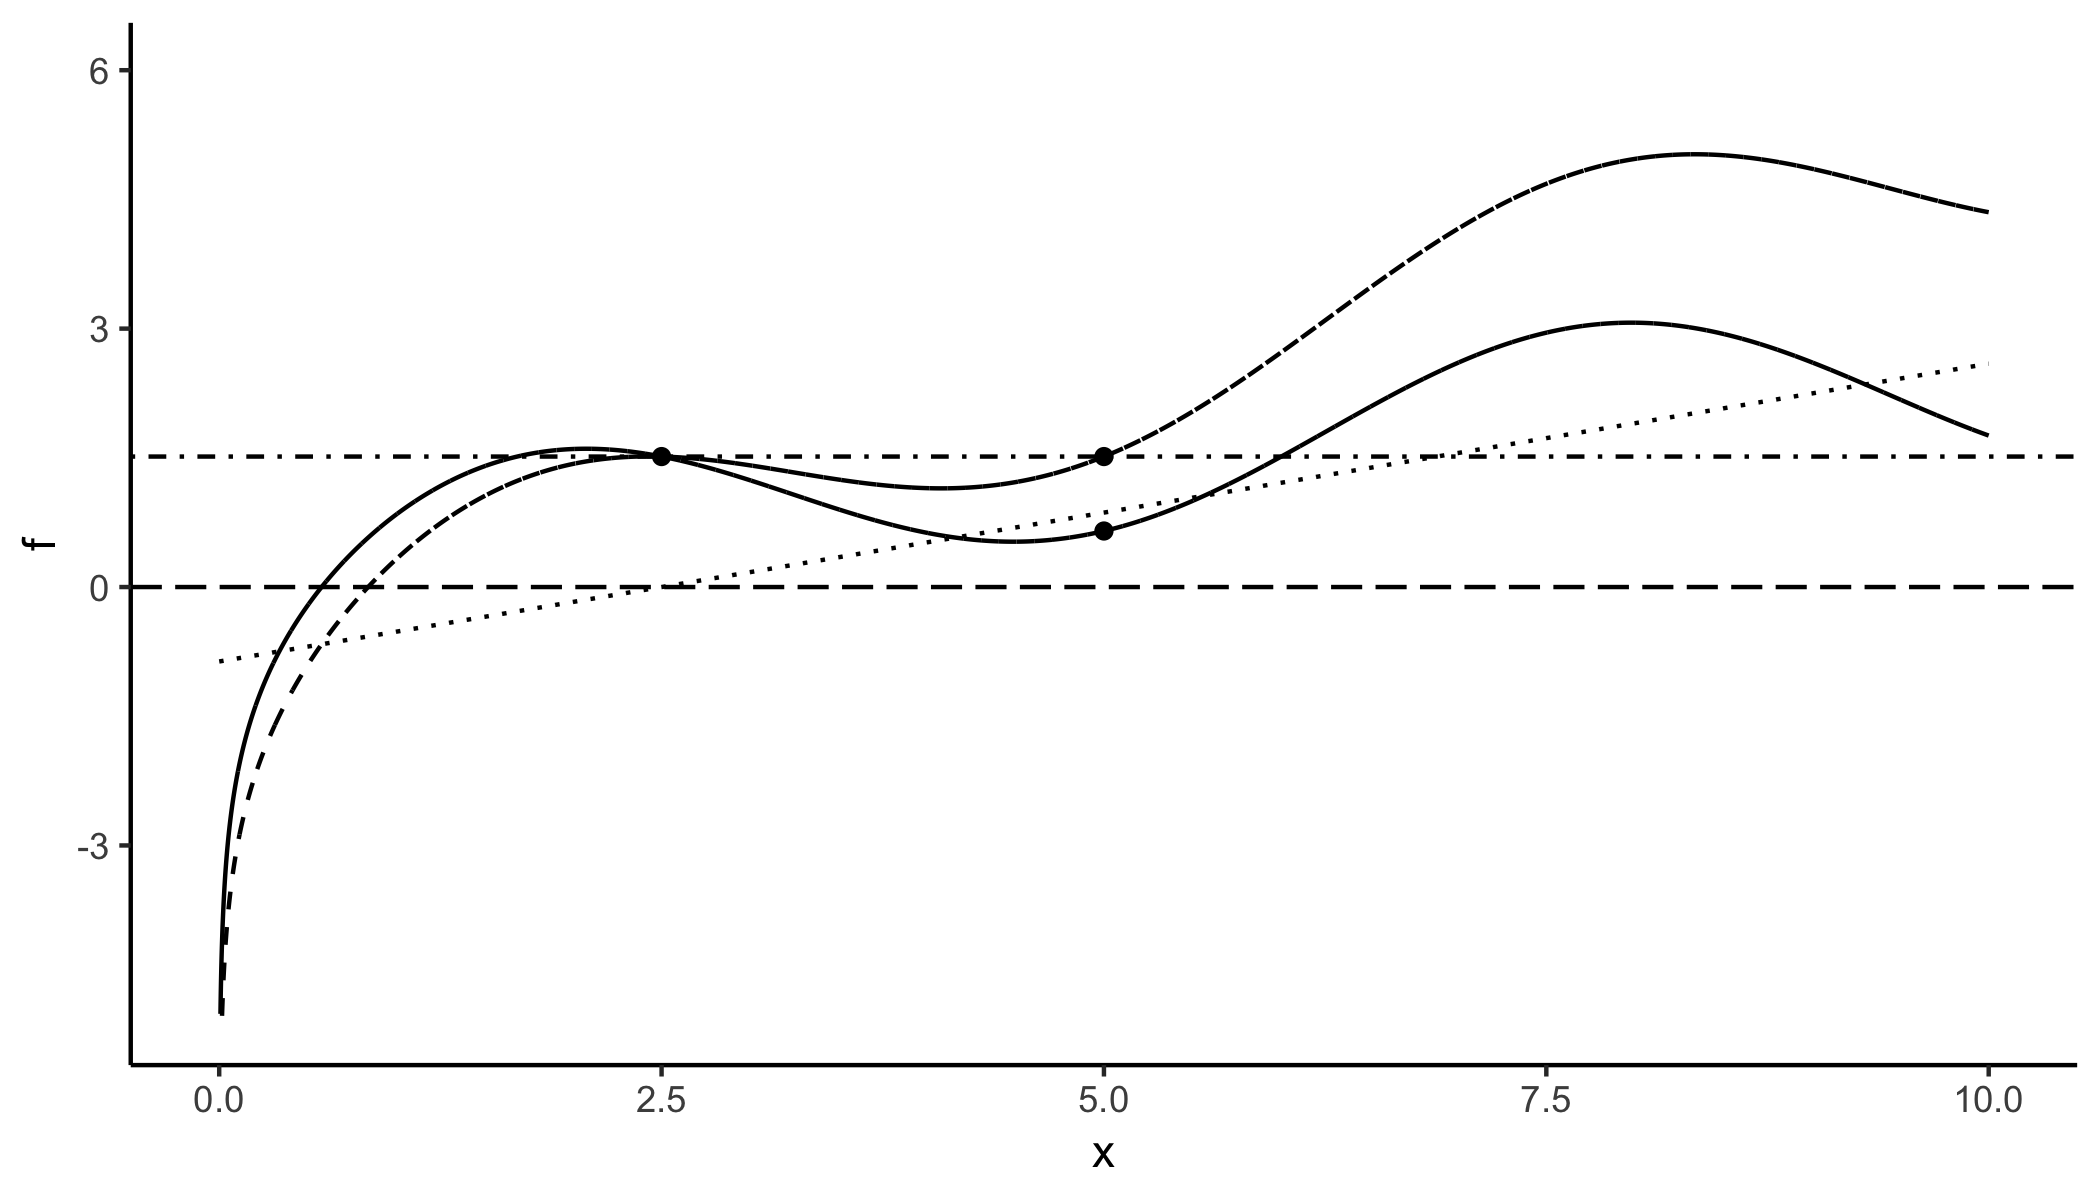
\includegraphics[width=3 in]{fig5.png}
\end{figure}
\end{frame}



\begin{frame}{Applying Rolle's Theorem}
$$g(x)=f(x)-\frac{(f(b)-f(a))}{b-a}(x-a)$$
$$g'(x)=0 \text{ at some c by Rolle's Theorem}$$\pause
$$g'(x)=f'(x)-\frac{(f(b)-f(a))}{b-a}$$\pause
$$g'(c)=0=f'(c)-\frac{(f(b)-f(a))}{b-a}$$\pause
$$f'(c)=\frac{(f(b)-f(a))}{b-a}$$

\end{frame}






\begin{frame}
\frametitle{Applications of Mean Value Theorem} 
\begin{itemize}
\item Speeding tickets: If the police can measure how long it takes me to get from point A to point B, at some point I was driving that speed.
\item Used to derive popular approximations to functions (including Taylor expansion)
\item We will use it in the proof of the Fundamental Theorem of Calculus relating derivatives to integrals.
\end{itemize}
\end{frame}

\begin{frame}

\begin{itemize}
\item \textcolor{mygray}{Derivative}
\item \textcolor{mygray}{Derivative Rules}
\item \textcolor{mygray}{Mean Value Theorem}
\item \textcolor{myblack}{Second Derivatives}
\end{itemize}

\end{frame}



\begin{frame}
\frametitle{Second Derivatives}

If the derivative is a slope, the second derivative is the slope of a slope.\pause

\frametitle{Second Derivatives}

\begin{defn} Suppose $f:\mathbb{R} \rightarrow \mathbb{R}$ is differentiable.  Recall we write this as $f^{'}$ and suppose that $f^{'}:\mathbb{R} \rightarrow \mathbb{R}$.  Then if the limit, 
\begin{eqnarray}
\lim_{x\rightarrow x_{0} } R(x) & = & \frac{f^{'}(x) - f^{'}(x_{0} ) } {x - x_{0} } \nonumber 
\end{eqnarray}
exists, we call this the \alert{second derivative} at $x_{0}, f^{''}(x_{0})$.  
\end{defn}

\end{frame}


\begin{frame}
\frametitle{Visualization of First and Second Derivative}


\begin{figure}[!ht]
\centering
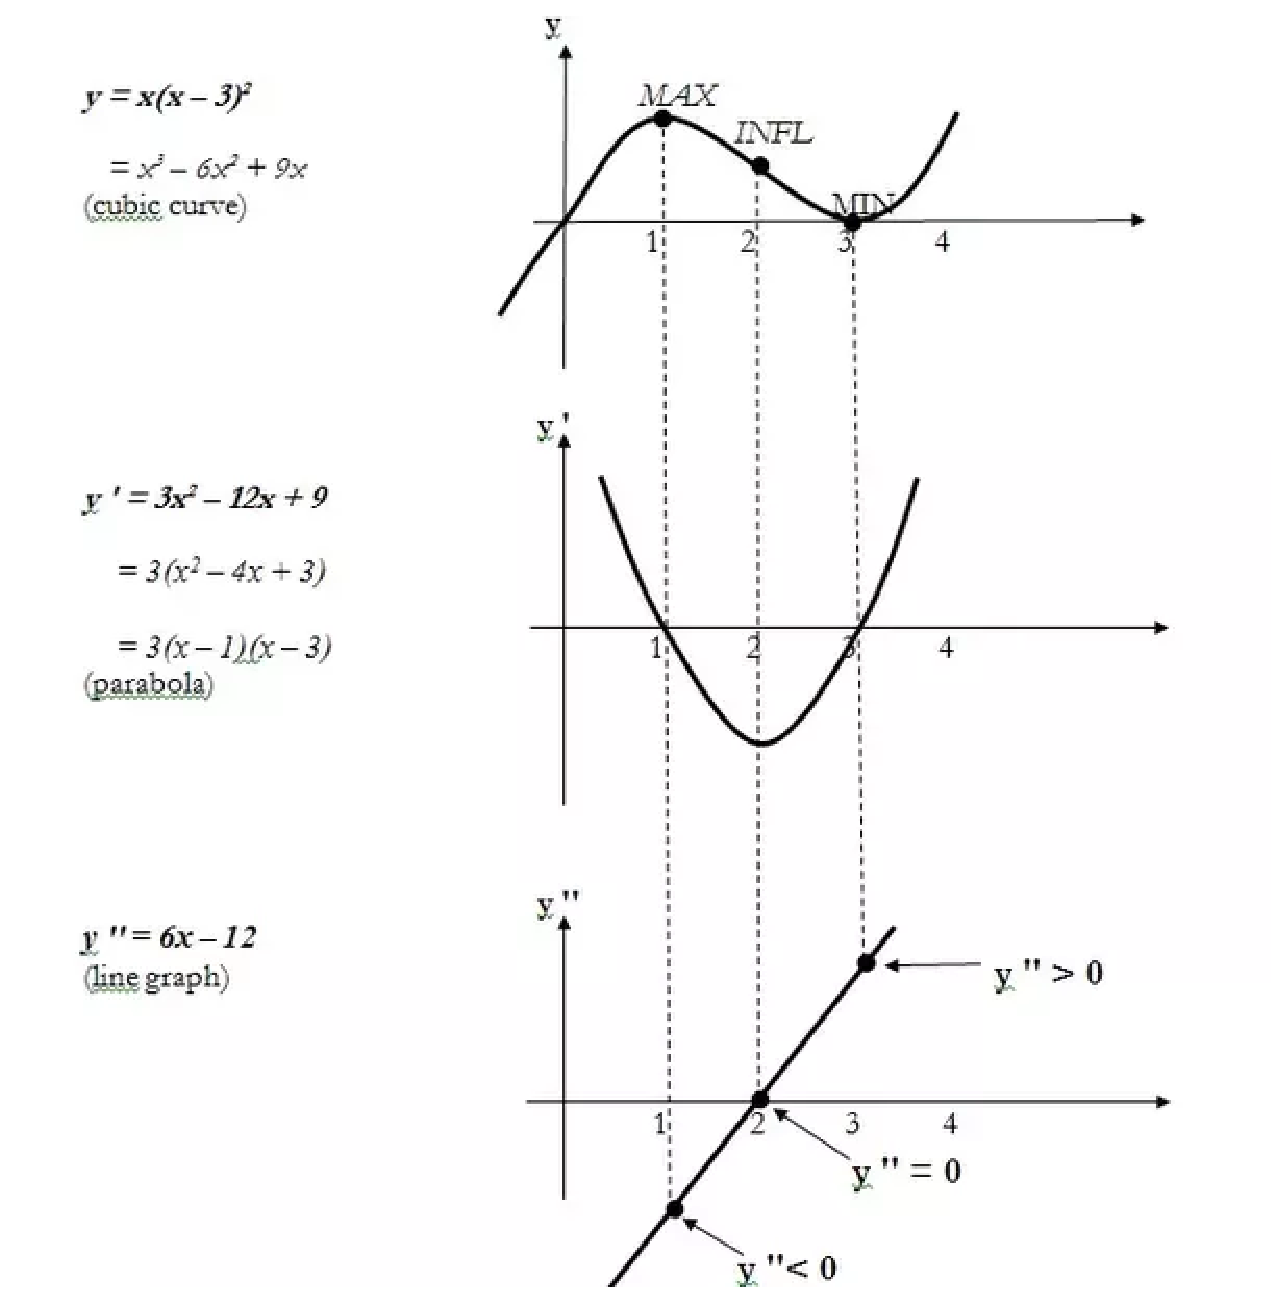
\includegraphics[scale = 0.3]{plsc43401_lec3_pic4}
\end{figure}

\end{frame}


\begin{frame}
\frametitle{Examples of Second Derivatives}

\only<1>{\begin{eqnarray}
f(x) & = & x \nonumber \\
f^{'}(x) & = & 1 \nonumber \\
f^{''} (x) & = & 0 \nonumber 
\end{eqnarray}}


\only<2>{\begin{eqnarray}
f(x) & = & e^{x} \nonumber \\
f^{'}(x) & = & e^{x} \nonumber \\
f^{''}(x) & = & e^{x} \nonumber
\end{eqnarray}}

\only<3>{
\begin{eqnarray}
f(x) & = & \log (x) \nonumber \\
f^{'}(x) & = & \frac{1}{x}=x^{-1} \nonumber \\
f^{''}(x) & = & -\frac{1}{x^2} \nonumber 
\end{eqnarray}
}

\only<4>{\begin{eqnarray}
f(x) & = & \frac{1}{x} \nonumber \\
f^{'}(x) & = & \frac{-1}{x^2} \nonumber \\
f^{''}(x) & = & \frac{2}{x^3} \nonumber 
\end{eqnarray}}


\only<5>{\begin{eqnarray}
f(x) & = & -x^2 + 20 \nonumber \\
f^{'}(x) & = & -2 x  \nonumber \\
f^{''}(x) & =& - 2 \nonumber 
\end{eqnarray}}
\end{frame}


\begin{frame}
\frametitle{Second Derivatives}

If the derivative is a slope, the second derivative is the slope of a slope.\pause

\frametitle{Second Derivatives}

\begin{defn} Suppose $f:\mathbb{R} \rightarrow \mathbb{R}$ is differentiable.  Recall we write this as $f^{'}$ and suppose that $f^{'}:\mathbb{R} \rightarrow \mathbb{R}$.  Then if the limit, 
\begin{eqnarray}
\lim_{x\rightarrow x_{0} } R(x) & = & \frac{f^{'}(x) - f^{'}(x_{0} ) } {x - x_{0} } \nonumber 
\end{eqnarray}
exists, we call this the \alert{second derivative} at $x_{0}, f^{''}(x_{0})$.  
\end{defn}

\end{frame}

\begin{frame}
\frametitle{Going forward}
\begin{itemize}
\item Your job is to memorize the product, quotient and chain rules of derivatives.
\item We will see how the second derivative is used to evaluate points as relative minima and maxima.
\end{itemize}
\end{frame}

\end{document}
